\chapter{\RRH\ Algorithm}
\label{chap:Reverse Rosu-Havelund Algorithm}

The reverse algorithm solves the shortcomings of the standard algorithm by changing the order in which the trace events are visited during evaluation.  The order is reversed to evaluate the trace from the earliest entry to the latest.  The effect of this is that when a new event occurs and the trace must be re-evaluated, that new evaluation always begins at the same event as the previous evaluation; the earliest event.

This is in contrast to the standard algorithm which visits the latest event first and moves backwards to the earliest event.  The problem is that the latest event is always different after a new event has occurred, so when evaluating a trace under the standard algorithm, that evaluation always begins from a new event.  This is a crucial detail because the standard algorithm involves the \textit{next} register.  The purpose of the \textit{next} register is to accumulate the evaluation result of each event in the trace as they are visited.  But at the moment when a new event occurs the result held in the \textit{next} register becomes invalid because it was determined before the new event happened.  Therefore, under the standard algorithm the \textit{next} register must be entirely redetermined every time a new event occurs, otherwise the final result of evaluating the trace will be incorrect.\\
\\
\section{Comparison Between Standard and Reverse Algorithms When Evaluating an Extending Trace}

To demonstrate the problem with the standard algorithm and the solution, we will compare the intermediate result of evaluating a trace that increases in length.  We will first use the standard, and then the reverse algorithm and show the intermediate result after each evaluation.  

\begin{myEx} Standard \RH\\
\\
\noindent
The \textit{next} register is defined as an intermediate result in a computational sequence that we wish to reuse between evaluations.\\
\\
\indent Let $t_1$ be a trace,\\
\indent as events occur $t_1$ is extended by one event,\\
\indent after the first event $t_1 =\ <e_1>$,\\
\indent after the second event $t_1 =\ <e_1, e_2>$,\\
\indent after n events $t_1 =\ <e_1 ... e_n>$.\\
\\
The computation sequence obtained when the $n^{th}$ event has occurred has a step for each suffix in the trace because the algorithm iterates from the last entry to the first:\\
\\$
\indent next(e_n),\\
\indent next(e_{n-1}, e_n),\\
\indent ...\\
\indent next(e_1 ... e_n)\\
\\
\indent intermediate\ result = next(e_1 ... e_n)\\
$\\
The result of the evaluation is the first element in the \textit{next} register.  The intermediate result is the \textit{next} register - $next(e_1 ... e_n)$.\\
\\
When a further event occurs the trace is extended to $t_2 =\ <e_1 ... e_n, e_{n+1}>$.  The computational sequence we would obtain from evaluating the  $t_2$ trace is:\\
\\$
\indent next(e_{n+1}),\\
\indent next(e_n, e_{n+1}),\\
\indent ...\\
\indent next(e_1 ... e_n, e_{n+1})\\
\\
\indent intermediate\ result = next(e_1 ... e_n, e_{n+1})\\
$\\
None of the steps performed to compute the intermediate result from $t_1$ contain $e_{n+1}$, yet all the computation steps performed to evaluate $t_2$ do.  There is no overlap between the computational sequences of the two evaluations thus it is impossible to reuse the \textit{next} register between evaluations.  Instead the register must be entirely recomputed after every new event so that it includes the evaluation of the $e_{n+1}$ event.
\\
\qed
\end{myEx}

To address this problem we rename the \textit{next} register to \textit{previous} to reflect the fact that it now stores the accumulated evaluations of all earlier events in the trace rather than later events.  Because all evaluations under the reverse algorithm start from the same event it means that even after a new event occurs the \textit{previous} register still holds a valid accumulation of all previous events.  Therefore it is not necessary to redetermine the \textit{previous} register every time a new event occurs.

\begin{myEx}\RRH\\
\\
Let $t_3$ be a trace of n events, $t_3 =\ <e_1 ... e_n>$.  The computation sequence we get when the $n^{th}$ event occurs has a step for each prefix of the trace because the reverse algorithm iterates from the first entry to the last:\\
\\$
\indent previous(e_1),\\
\indent previous(e_1, e_2),\\
\indent ...\\
\indent previous(e_1 ... e_n)\\
\\
\indent intermediate\ result = previous(e_1 ... e_n)$\\
\\
\noindent 
When a further event occurs, the trace is extended to $t_4 =\ <e_1 ... e_n, e_{n+1}>$.  The computational sequence we obtain is:\\
\\$
\indent previous(e_1),\\
\indent previous(e_1, e_2),\\
\indent ...\\
\indent previous(e_1 ... e_n),\\
\indent previous(e_1 ... e_n, e_{n+1})\\
\\
\indent intermediate\ result = previous(e_1 ... e_n, e_{n+1})\\
$\\
We can see the computational sequences do overlap.  The only step that was performed for $t_4$ and not for $t_3$ is the last step, $previous(e_1 ... e_n, e_{n+1})$, that corresponds to the new event.  This means the intermediate result of evaluating $t_3$ is the same result we arrive at after all but the final computational step for $t_4$.  Therefore we can reuse the \textit{previous} register between evaluations without recomputing it.  The only computational step that must get performed to evaluate $t_4$ is the final step that evaluates the formula over the new event.\\
\qed
\end{myEx}

\section{Consequences of Reverse Evaluation}

When we make these changes to the algorithm, the effect is that we do not need to visit every event in the trace whenever a new event occurs.  The \textit{previous} register already holds the cumulative outcome of evaluating all earlier events in the trace, so if the evaluation of a new event calls for us to refer to the evaluation result of a previous event then we can refer the \textit{previous} register without additional computational cost.  Therefore, whenever an event occurs only that single event has to be visited rather than the whole trace.

While this is a substantial complexity improvement over the standard algorithm, it comes at an expense.  A problem arises when evaluating the future LTL operators; until, eventually, and next.  The semantics of the future LTL operators refer to the evaluations of events following the event being evaluated.  But, when the latest event is being evaluated, the future events are not known.  It is therefore impossible to evaluate formulae that include future LTL operators.

This is not a disaster because having the \textit{previous} register at hand means it is possible to evaluate LTL formulae written in terms of past events.  The reverse algorithm replaces the future LTL operators defined in sections \ref{sec:LTLFutureGrammar} and \ref{sec:LTLFutureSemantics} with the past LTL operators; once, previous and has-always-been; defined in \ref{sec:LTLPastGrammar} and \ref{sec:LTLPastSemantics}.

We make the conjecture that any security property we wish to formulate, can be written in terms of past events and past operators.  For example, a policy might be that there should be no audio taken from the microphone if there are no calls in progress.  In that case we would formulate a property that is satisfied when an audio read event \textit{has} taken place, and there were no \textit{preceding} call events.  Such a property is concerned with events occurring in the past.  We assert that all security properties can be written in this manner.  We support this conjecture by calling upon Pneuli's description of the past termporal operators.  He describes the past operators as `a symmetric counterpart to each of the future operators.  While the future formula describes a property holding at a suffix of the model (...), a past formula describes a property of a prefix of the model'\footnote{The Temporal Logic of Reactive and Concurrent Systems, Manna and Pneuli, section 3.3}.  Indeed, the difference between the standard algorithm and the reverse algorithm is that the semantics of the future operators operate upon the trace suffix and the past operators upon the prefix.\\
\\
\noindent
The upshot is that the collusion property we formulated in chapter \ref{chap:Monitoring For Security Properties} as $\LTLeventually(q \land \LTLeventually(s \land \LTLeventually(r \land \LTLeventually p)))$, must be altered to define the property in terms of past events rather than future.  In future parlance the property reads `eventually there is a query and eventually there is a send and eventually there is a receive and eventually there is a publish'.  We reformulate this to read `once there was a publish and once there was a receive and once there was a send and once there was a query'.  Written as LTL the eventually operator, $\LTLeventually$, is swapped for the once operator, $\LTLonce$, and the order of the events is reversed.  The formula then appears:\\

$$\LTLonce(p \land \LTLonce(r \land \LTLonce(s \land \LTLonce q)))$$\\  

\begin{myEx} Collusion Formula Examples\\

Examples of the collusion formula evaluated over a positive and negative trace are in appendix \ref{app:PastLogicCollusionFormulaExamples}.

\qed
\end{myEx}

%\section{Correctness Proof Of Reverse Ro\c{s}u-Havelund Algorithm}
%\label{sec:Scalability Of Reverse Rosu-Havelund Algorithm}

% TODO

\section{Implementation of \RRH\ Algorithm}
\label{sec:Implementation Of Reverse Rosu-Havelund Algorithm}

The algorithm is implemented within the monitor process shown in the high level architecture diagram \ref{fig:highLevelArchitectureDiagram}, on page \pageref{fig:highLevelArchitectureDiagram}.  The structure of the monitor process is illustrated in class diagram \ref{fig:eventReceiverClassDiagram} and in greater detail in \ref{fig:monitorClassDiagram}.

%Event Receiver Class Diagram
\begin{figure}[h]
	\centering
	\begin{tikzpicture}[scale=0.7, every node/.style={transform shape}]
	\umlsimpleclass[alias=BroadcastReceiver]{android.content::BroadcastReceiver (abstract)}
	\umlclass[alias=EventReceiver, x=0, y=-3]{com.androidmonitor::EventReceiver}{}{+onReceive(context: Context, intent: Intent): void}
	\umlsimpleclass[alias=monitors, x=0, y=-6]{java.util::ArrayList$<$Monitor$>$}
	\umlclass[alias=Monitor, x=0, y=-9]{RosuHavelund::Monitor}
		{}
		{
			+Evaluate(traceEvent: TraceEvent): EvaluationResult\\
			+Reset(): void
		}
	
	\umlinherit{EventReceiver}{BroadcastReceiver}
	\umlcompo[mult1=1, arg2=-monitors, mult2=1]{EventReceiver}{monitors}
	\umluniassoc[mult2=0..n]{monitors}{Monitor}
	
	\umlclass[alias=EvaluationResult, x=9, y=-1]{RosuHavelund::EvaluationResult}
		{}
		{
			+Satisfied():boolean\\
			+Message(): String\\
			+SatisfyingEvents() ArrayList$<$TraceEvent$>$
		}
	\umlsimpleclass[alias=satisfyingEvents, x=9, y=-5]{java.util::ArrayList$<$TraceEvent$>$}
	\umlclass[alias=TraceEvent, x=9, y=-9]{RosuHavelund::TraceEvent}
		{}
		{
			+Time():Date\\
			+Event(): String\\
			+Pid(): Int\\
			+AppName(): String\\
			+Action(): String\\
		}

	\umlcompo[mult1=1, arg2=-satisfyingEvents, mult2=1]{EvaluationResult}{satisfyingEvents}
	\umluniassoc[mult2=0..n]{satisfyingEvents}{TraceEvent}

	\end{tikzpicture}
	\caption{Event Receiver Class Diagram}
	\label{fig:eventReceiverClassDiagram}
\end{figure}

The reader can observe that there is a monitor class composed of two registers, \textit{now} and \textit{previous}, and that registers are an array of expressions.\\
\\
There are two phases of the algorithm to explain:

\begin{enumerate}
\item Initialisation %Initialisation is the construction of registers from an LTL formula.   
\item Evaluation %Iterating through a trace evaluating the formula over an event from that trace.
\end{enumerate}

\subsection{Initialisation}
\label{sec:Initialisation}

The \RH\ algorithm constructs breadth-first ordered arrays they call registers, where the first element is the root, and successive elements correspond to deeper subformulae.  An important consideration is that the subformulae of a given formula are not always immediately adjacent to the root in the register.\\
\\
The following example illustrates this consideration:

\begin{myEx} The formula $ \varphi = \LTLalwaysbeen((p \,S \,q) \rightarrow \LTLonce(q \rightarrow \LTLprevious r)) $ produces subformulae:
\begin{flushleft}
$ \varphi_{1} = \LTLalwaysbeen((p \,S \,q) \rightarrow \LTLonce(q \rightarrow \LTLprevious r)) $ \\
$ \varphi_{2} = ((p \,S \,q) \rightarrow \LTLonce(q \rightarrow \LTLprevious r)) $ \\
$ \varphi_{3} = (p \,S \,q) $ \\
$ \varphi_{4} = \LTLonce(q \rightarrow \LTLprevious r) $ \\
$ \varphi_{5} = p $ \\
$ \varphi_{6} = q $ \\
$ \varphi_{7} = (q \rightarrow \LTLprevious r) $ \\
$ \varphi_{8} = q $ \\
$ \varphi_{9} = \LTLprevious r $ \\
$ \varphi_{10} = r $ 
\end{flushleft}

\noindent
When arranged in breadth-first order in an array they appear:

\begin{tabularx}{\textwidth}{cc|c|c|c|c|c|c|c|c|c|c|}
\centering
 & \multicolumn{1}{c}{}
 & \multicolumn{1}{c}{$ \varphi_{1}$}
 & \multicolumn{1}{c}{$ \varphi_{2}$}
 & \multicolumn{1}{c}{$ \varphi_{3}$}
 & \multicolumn{1}{c}{$ \varphi_{4}$}
 & \multicolumn{1}{c}{$ \varphi_{5}$}
 & \multicolumn{1}{c}{$ \varphi_{6}$}
 & \multicolumn{1}{c}{$ \varphi_{7}$}
 & \multicolumn{1}{c}{$ \varphi_{8}$}
 & \multicolumn{1}{c}{$ \varphi_{9}$}
 & \multicolumn{1}{c}{$ \varphi_{10}$}\\
 \cline{3-12}
 & {now} 
 & { \tikz[baseline]{\node (p1) {$\LTLalwaysbeen$};} } 
 & { \tikz[baseline]{\node (p2) {$\rightarrow$};} }  
 & { \tikz[baseline]{\node (p3) {$ S $};} }
 & { \tikz[baseline]{\node (p4) {$\LTLonce$};} }
 & { \tikz[baseline]{\node (p5) {$p$};} }
 & { \tikz[baseline]{\node (p6) {$q$};} }
 & { \tikz[baseline]{\node (p7) {$\rightarrow$};} }
 & { \tikz[baseline]{\node (p8) {$q$};} }
 & { \tikz[baseline]{\node (p9) {$\LTLprevious$};} }
 & { \tikz[baseline]{\node (p10) {$r$};} } \\
 \cline{3-12}
\end{tabularx}
\begin{tikzpicture}[overlay]
    \draw[red, thick,->] (p1) edge[bend left=10] (p2);
    \draw[red, thick,->] (p2) edge[bend left=10] (p3);
    \draw[red, thick,->] (p2) edge[bend right=30] (p4);
    \draw[red, thick,->] (p3) edge[bend left=30]  (p5);
    \draw[red, thick,->] (p3) edge[bend right=30] (p6);
    \draw[red, thick,->] (p4)[bend left=20] edge (p7);
    \draw[red, thick,->] (p7)[bend left=10] edge (p8);
    \draw[red, thick,->] (p7)[bend right=30] edge (p9);
    \draw[red, thick,->] (p9)[bend left=10] edge (p10);
\end{tikzpicture}
\qed
\end{myEx}

The arrows indicate which elements in the register are the operands of another element.  We can see the first element, $\varphi_1$, is the unary has-always-been operator at the root.  In that case, its operand is indeed the adjacent element $\varphi_2$.  But $\varphi_2$ is a binary implies formula with two subformulae as operands.  The satisfaction of $\varphi_2$ is dependent on the immediately adjacent $\varphi_3$ and also on the next element $\varphi_4$.  And the satisfaction of $\varphi_4$ depends on the satisfaction of $\varphi_7$.  To reference the subformulae of a formula is not a trivial exercise of simply referencing the adjacent element in the register.  Instead, the element corresponding to that subformula may be any of the following elements.  When evaluating each element within the register, the challenge is finding the elements corresponding to the operands.

%Monitor Class Diagram
\begin{figure}[h]
	\centering
	\begin{tikzpicture}[scale=0.65, every node/.style={transform shape}]

		\umlclass[alias=Monitor, x=0, y=0]{RosuHavelund::Monitor}
		{}
		{
			+Evaluate(traceEvent: TraceEvent): EvaluationResult\\
			+Reset(): void
		}
		
	\umlclass[alias=DynamicConditions, x=12, y=0]{RosuHavelund::DynamicConditions}
		{}
		{
			\umlvirt{\#Met(satisfyingEvents: ArrayList$<$TraceEvent$>$): ArrayList$<$TraceEvent$>$}
		}

	\umlclass[alias=CollusionConditions, x=12, y=-4]{RosuHavelund::CollusionConditions}
		{}
		{
			+Met(satisfyingEvents: ArrayList$<$TraceEvent$>$): ArrayList$<$TraceEvent$>$\\
		}

	\umlclass[alias=Register, x=0, y=-5]{RosuHavelund::Register}
		{}
		{
			+Evaluate(event: String): boolean\\
			+Satisfied(): boolean\\
			+Update(register: Register): void\\
			+Reset(): void
		}

	\umlsimpleclass[alias=expressions, x=0, y=-9]{java.util::ArrayList$<$Expressions$>$}

	\umlclass[alias=Expression, x=0, y=-14]{RosuHavelund::Expression (abstract)}
		{
			+Formula(): String\\
			+Previous(): Expression\\
			+Satisfied(): boolean\\
		}
		{
			+Evaluate(event: String): boolean\\
			+setSatisfied(satisfied: boolean)\\
			+Reset(): void\\
			+FlattenBreadthFirst(): ArrayList$<$Expression$>$
		}
		
	\umlinherit{CollusionConditions}{DynamicConditions}
	\umlcompo[mult1=1, arg2=-now, mult2=1, anchor1=-130, anchor2=120]{Monitor}{Register}
	\umlcompo[mult1=1, arg2=-previous, mult2=1, anchor1=-50, anchor2=60]{Monitor}{Register}
	\umlcompo[mult1=1, arg2=-dynamicConditions, pos2=0.7, mult2=1]{Monitor}{CollusionConditions}
	\umlcompo[mult1=1, arg2=-expressions, mult2=1]{Register}{expressions}
	\umluniassoc[mult2=0..n]{expressions}{Expression}

	\end{tikzpicture}
  \caption{Monitor Class Diagram}
  \label{fig:monitorClassDiagram}
\end{figure}

The solution is to make each element of the register a composition that we call an expression.  Expressions follow a hierarchical structure shown in the class diagram \ref{fig:expressionHeirarchy}.  They are either literals that have no operator or operands, unary expressions with an operator and a single operand, or binary expressions that have an operator and two operands. An expression is composed of a formula string, a boolean that tells us if the result of evaluating an event satisfies the formula, and references to operand expressions elsewhere in the register.

% Expression Hierarchy Class Diagram
\begin{figure}[h!]
	\centering
	\begin{tikzpicture}[scale=0.55, every node/.style={transform shape}]
	
		\umlclass[alias=Expression, x=-8, y=0]{RosuHavelund::Expression (abstract)}
		{
			+Formula(): String\\
			+Previous(): Expression\\
			+Satisfied(): boolean\\
		}
		{
			+Evaluate(event: String): boolean\\
			+setSatisfied(satisfied: boolean)\\
			+Reset(): void\\
			+FlattenBreadthFirst(): ArrayList$<$Expression$>$
		}

		\umlclass[alias=UnaryExpression, x=-2, y=-5]{RosuHavelund::UnaryExpression (abstract)}
		{
			+Operator(): String\\
			+LeftOperand(): Expression\\
		}
		{}
		\umlinherit[geometry=-|]{UnaryExpression}{Expression}

		\umlclass[alias=LiteralExpression, x=-13, y=-5]{RosuHavelund::LiteralExpression}
		{}
		{
			\umlstatic{+Match(formula: String): boolean}\\
			\umlstatic{+MatchPosition(formula: String): int}\\
		}
		\umlinherit[geometry=-|]{LiteralExpression}{Expression}

		\umlclass[alias=BinaryExpression, x=2, y=-9]{RosuHavelund::BinaryExpression (abstract)}
		{
			+RightOperand(): Expression\\
		}
		{}
		\umlinherit[geometry=-|, anchors=180 and -140]{BinaryExpression}{UnaryExpression}

		\umlclass[alias=NotExpression, x=-9, y=-9]{RosuHavelund::NotExpression}
		{}
		{
			\umlstatic{+Match(formula: String): boolean}\\
			\umlstatic{+MatchPosition(formula: String): int}\\
		}
		\umlinherit[geometry=-|, anchors=0 and -140]{NotExpression}{UnaryExpression}

		\umlclass[alias=AlwaysBeenExpression, x=-9, y=-13]{RosuHavelund::AlwaysBeenExpression}
		{}
		{
			\umlstatic{+Match(formula: String): boolean}\\
			\umlstatic{+MatchPosition(formula: String): int}\\
		}
		\umlinherit[geometry=-|, anchors=0 and -140]{AlwaysBeenExpression}{UnaryExpression}

		\umlclass[alias=OnceExpression, x=-9, y=-17]{RosuHavelund::OnceExpression}
		{}
		{
			\umlstatic{+Match(formula: String): boolean}\\
			\umlstatic{+MatchPosition(formula: String): int}\\
		}
		\umlinherit[geometry=-|, anchors=0 and -140]{OnceExpression}{UnaryExpression}

		\umlclass[alias=PreviousExpression, x=-9, y=-21]{RosuHavelund::PreviousExpression}
		{}
		{
			\umlstatic{+Match(formula: String): boolean}\\
			\umlstatic{+MatchPosition(formula: String): int}\\
		}
		\umlinherit[geometry=-|, anchors=0 and -140]{PreviousExpression}{UnaryExpression}
	
		\umlclass[alias=AndExpression, x=6, y=-13]{RosuHavelund::AndExpression}
		{}
		{
			\umlstatic{+Match(formula: String): boolean}\\
			\umlstatic{+MatchPosition(formula: String): int}\\
		}
		\umlinherit[geometry=-|, anchors=180 and -140]{AndExpression}{BinaryExpression}

		\umlclass[alias=OrExpression, x=6, y=-17]{RosuHavelund::OrExpression}
		{}
		{
			\umlstatic{+Match(formula: String): boolean}\\
			\umlstatic{+MatchPosition(formula: String): int}\\
		}
		\umlinherit[geometry=-|, anchors=180 and -140]{OrExpression}{BinaryExpression}

		\umlclass[alias=ImpliesExpression, x=6, y=-21]{RosuHavelund::ImpliesExpression}
		{}
		{
			\umlstatic{+Match(formula: String): boolean}\\
			\umlstatic{+MatchPosition(formula: String): int}\\
		}
		\umlinherit[geometry=-|, anchors=180 and -140]{ImpliesExpression}{BinaryExpression}
		
		\umlclass[alias=SinceExpression, x=6, y=-25]{RosuHavelund::SinceExpression}
		{}
		{
			\umlstatic{+Match(formula: String): boolean}\\
			\umlstatic{+MatchPosition(formula: String): int}\\
		}
		\umlinherit[geometry=-|, anchors=180 and -140]{SinceExpression}{BinaryExpression}
	\end{tikzpicture}
 	\caption{Expression Heirarchy}
 	\label{fig:expressionHeirarchy}
\end{figure}

Each register gets constructed from a syntax tree.  The syntax tree gets constructed first by recursively parsing an LTL formula string.  Nodes in a syntax tree are instances of the expression subclasses in figure \ref{fig:expressionHeirarchy}.

Trees get constructed by a class factory that contains all the concrete subclasses of the expression class.  The class factory returns an instance of the expression whose operator corresponds to the root operator of the formula it gets passed.  It does this by iterating through the registered expressions, calling the static match method on each, until it finds the one whose operator matches the outermost\footnote{The outermost operator gets identified as the operator outside all braces} operator of the formula.  The match method is static because we do not wish to construct an instance of the class only to discover the operator does not match the operator of the formula.  When the matching expression gets found, the class factory constructs an instance and passes the formula to the constructor.  The expression constructor identifies the formula operands as the substrings to the left and right of the outermost operator.  It constructs child expressions for the operands by calling the class factory again with each operand string.  The process recurses until it reaches leaf nodes with no operator or operands.  At this point, the class factory constructs a literal class with no further child nodes.  The syntax tree is complete.

The \textit{now} and \textit{previous} registers get created from the resulting tree structures by flattening each tree into a breadth-first ordered array of expressions.  There is a flatten method on the root node of each tree that traverses the tree in breadth-first order, putting each node in an array.  As mentioned earlier, the operands of each expression are references to child expressions in the tree.  Once the tree gets flattened into an array, the references point to other array elements.  Then it is easy to reach operands elsewhere in the register.

The semantics of the temporal operators, such as has-always-been and once, involve earlier evaluations.  The \textit{previous} register keeps track of earlier evaluations, therefore the \textit{now} register needs a reference to it.  The syntax tree for the \textit{previous} register gets constructed first, and the root expression gets passed to the constructor of the \textit{now} tree.  As each node in the \textit{now} tree is constructed, the \textit{previous} tree is traversed in unison.  A reference to the corresponding node from the \textit{previous} tree is passed to the constructor of each \textit{now} tree node and held.  The reference is called Previous and can be seen in the Expression class in figures \ref{fig:monitorClassDiagram} and \ref{fig:expressionHeirarchy}. When the trees get flattened into registers, the expressions from the \textit{previous} register are available to the corresponding expressions in the \textit{now} register during evaluation.

% Event evaluation sequence diagram
\begin{figure}[h]
	\begin{resizedtikzpicture}{\textwidth}
		\begin{umlseqdiag}
		\umlactor[class=Process]{app}
		\umlobject[class=Interceptor]{interceptor}
		\umlactor[class=Process]{monitorProcess}
		\umlobject[class=EventReceiver]{receiver}
		\umlmulti[class=Monitor]{monitor}
		\umlmulti[class=Register]{register}
		\umlmulti[class=Expression]{expression}
		\umlobject[class=CollusionConditions, x=30]{dynamicConditions}
		\begin{umlcall}[op={action}]{app}{interceptor}
			\begin{umlcall}[op={intent}]{interceptor}{monitorProcess}
				\begin{umlcall}[op={onReceive(intent)}]{monitorProcess}{receiver}
		
					\begin{umlfragment}[type=loop, label=foreach monitor]
					
						\begin{umlcall}[op={Evaluate(event)}, return=result]{receiver}{monitor}
							\begin{umlcall}[op={now.Evaluate(event)}, return=result]{monitor}{register}
								\begin{umlfragment}[type=loop, label=foreach expression, inner xsep=7]
									\begin{umlcall}[op={Evaluate(event)}, return=result]{register}{expression}\end{umlcall}
								\end{umlfragment}
							\end{umlcall}
							\begin{umlcall}[op={previous.Update()}]{monitor}{register}\end{umlcall}
							
							\begin{umlfragment}[type=opt, label=if previous.Satisfied, inner xsep=7]
								\begin{umlcall}[op={Met(satisfyingEvents)}, return=satisfyingEvents]{monitor}{dynamicConditions}\end{umlcall}			
							\end{umlfragment}
						\end{umlcall}
					
						\begin{umlfragment}[type=opt, label=if result.Satisfied, inner xsep=4]
							\begin{umlcall}[op={Reset()}]{receiver}{monitor}
								\begin{umlcall}[op={now.Reset()}]{monitor}{register}
									\begin{umlfragment}[type=loop, label=foreach expression, inner xsep=7]
										\begin{umlcall}[op={Reset()}]{register}{expression}\end{umlcall}
									\end{umlfragment}
								\end{umlcall}
								
								\begin{umlcall}[op={previous.Reset()}]{monitor}{register}
									\begin{umlfragment}[type=loop, label=foreach expression, inner xsep=7]
										\begin{umlcall}[op={Reset()}]{register}{expression}\end{umlcall}
									\end{umlfragment}
								\end{umlcall}
							\end{umlcall}
						\end{umlfragment}
						
					\end{umlfragment}
			\end{umlcall}
			\end{umlcall}
		\end{umlcall}
		\end{umlseqdiag}
	\end{resizedtikzpicture}
    \caption{Evaluation of an Action}
    \label{fig:monitorSequenceDiagram}
\end{figure}

\subsection{Evaluation}
\label{sec:Evaluation}

The sequence diagram \ref{fig:monitorSequenceDiagram} illustrates the evaluation of an event in detail.  The monitor process receives an event from the interceptor in the EventReceiver class.  EventReceiver has a collection of monitor instances where each instance monitors for a different formula.

The event gets evaluated by calling the evaluate method on each monitor and passing the event as a parameter.  The monitor evaluates the event by iterating through each expression in the \textit{now} register.  It goes from the last expression to the first, calling their evaluate method and passing the event.  Each expression class implements the LTL semantics in \ref{def:PastNon-emptyTraceSemantics} that define the expressions operator.  If the event satisfies an expression, then the monitor adds it to a list of satisfying events.  The result of the monitor evaluate method is an EvaluationResult.  It comprises a boolean to indicate satisfaction of the formula, and the list of events that contributed to satisfaction.

In a similar fashion to the \RH\ implementation, implementing the semantics for each operator is a case of replacing terms from that operator's semantic statement with references to their implementation counterparts.  Subformulae of $\varphi$ are replaced with elements within the \textit{now} and \textit{previous} registers by the use of indices $i$, $j$ and $k$.  The index $i$ maps to the element corresponding to the subformulas operator.  Indices $j$ and $k$ map to the elements corresponding to the left and right operands respectively.\\
\\
For a given trace event $e$, for all $i$ ranging from length(\textit{now})..1, if the $i^{th}$ outermost operator is:

\begin{enumerate}
\item literal l, then \textit{now}[$i$] $\leftarrow$ (l == $e$)
\item $ \neg $ then \textit{now}[$i$] $ \leftarrow $ NOT(\textit{now}[$j$]).
\item $ \lor $ then \textit{now}[$i$] $ \leftarrow $ \textit{now}[$j$] OR \textit{now}[$k$]. 
\item $ \land $ then \textit{now}[$i$] $ \leftarrow $ \textit{now}[$j$] AND \textit{now}[$k$]. 
\item $ \rightarrow $ then \textit{now}[$i$] $ \leftarrow $ NOT(\textit{now}[$j$]) OR \textit{now}[$k$]. 
\item $ \LTLprevious $ then \textit{now}[$i$] $ \leftarrow $ \textit{previous}[$j$].
\item $ \LTLalwaysbeen $ then \textit{now}[$i$] $ \leftarrow $ \textit{now}[$j$] AND \textit{previous}[$i$].
\item $ \LTLonce $ then \textit{now}[$i$] $ \leftarrow $ \textit{now}[$j$] OR \textit{previous}[$i$].
\item S then \textit{now}[$i$] $ \leftarrow $ \textit{now}[$k$] OR (\textit{now}[$j$] AND \textit{previous}[$i$]).
\end{enumerate}

When the monitor has evaluated the event over the \textit{now} register, it accumulates the result into the \textit{previous} register by calling its update method.  The satisfaction of each \textit{previous} register expression is set to that of the corresponding \textit{now} register expression.

Satisfaction of the first element, the root formula, in the \textit{previous} register indicates the final result of evaluating the event.

\section{Testing the \RRH\ Algorithm}
\label{sec:Testing The Reverse Rosu-Havelund Algorithm}

We performed similar functional tests on the reverse algorithm to those for the standard \RH\ algorithm, except that tests for future operators got replaced with tests for past operators.

Test cases got generated manually by applying the semantics of each operator, from section \ref{sec:LTLPastSemantics} to a series of traces and noting the expected result.  The test cases are in appendix \ref{app:RRHFunctionalTestCases}.  For practical use, it was necessary to replace some of the LTL symbols with characters available on the keyboard.  Table \ref{tab:AlternativeLTLOperators} provides the translation.

The tests were run by entering the formula and test traces from each test case into a test harness application.  The test harness then evaluated the formula over each trace using the \RRH\ implementation and wrote the results to the console window.  The results are in appendix \ref{app:RRHFunctionalTestResults} and the test harness code is in \ref{app:RRHCode}.  The results confirm the functionality is identical to that of the standard algorithm with respect to the classical logical operators and the functioning of the past temporal operators is as expected.

We also ran the same performance tests as those in section \ref{subsec:PracticalPerformanceAnalysisExecution} on the \RRH\ algorithm.  We used the reader and publisher apps to generate traces of increasing length and measured the time taken to evaluate each trace.

\subsection{Test Results}
\label{subsec:PracticalPerformanceAnalysisResultsRRH}

Table \ref{tab:ReverseRHExecutionTimes} gives the performance test results.  The time taken to evaluate each trace remained constant at less than a second, regardless of the size of the trace.

\begin{table}[h!]
	\centering
	\captionsetup{width=0.6\linewidth, justification=centering}
	\begin{tabular}{r|r} 
	Trace Length  & Duration\\
	(collusion sequences) & (seconds)\\
	\hline
	10 & $<1$\\
	20 & $<1$\\
	30 & $<1$\\
	40 & $<1$\\
	50 & $<1$\\
	60 & $<1$\\
	70 & $<1$\\
	80 & $<1$\\
	90 & $<1$\\
	100 & $<1$\\
	\hline
	\end{tabular}
	\caption{Duration of the \RRH\ Algorithm Evaluating Traces of Increasing Length}
	\label{tab:ReverseRHExecutionTimes}
\end{table}

\newpage

\section{Scalability of \RRH\ Algorithm}
\label{sec:Scalability Of Reverse Rosu-Havelund Algorithm}

Figure \ref{fig:ReverseRHEvaluationDuration} compares the performance of the standard \RH\ algorithm, plotted by the blue curve, with that of the \RRH\ algorithm, plotted by the flat green curve.  The results are in line with our expectations of the reverse algorithm and support its suitability for realtime monitoring.

\begin{figure}[h!]
	\centering
	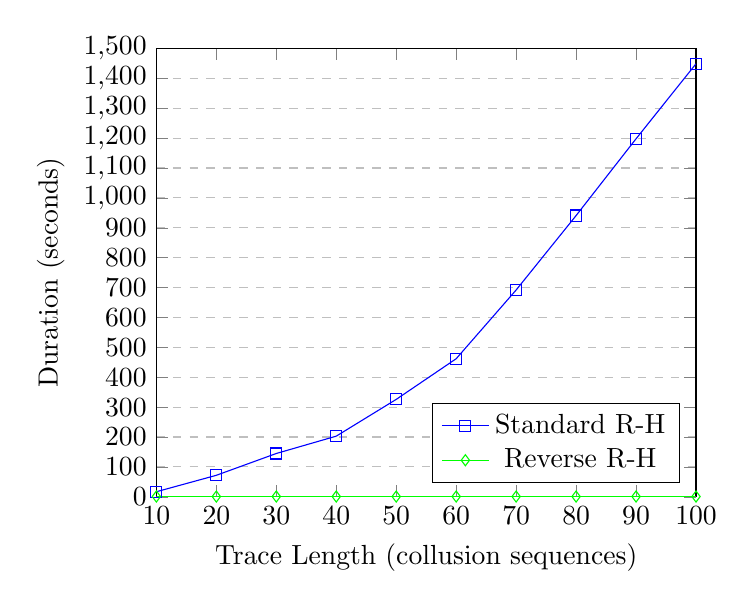
\begin{tikzpicture}
	\begin{axis}[
	    xlabel={Trace Length (collusion sequences)},
	    ylabel={Duration (seconds)},
	    xmin=10, xmax=100,
	    ymin=0, ymax=1500,
	    xtick={10,20,30,40,50,60,70,80,90,100},
	    ytick={0,100,200,300,400,500,600,700,800,900,1000,1100,1200,1300,1400,1500},
	    legend pos=south east,
	    ymajorgrids=true,
	    grid style=dashed,
	]
	
	\addplot[
	    color=blue,
	    mark=square,
	    ]
	    coordinates {
	    (10,17)(20,72)(30,145)(40,203)(50,326)(60,462)(70,692)(80,941)(90,1198)(100,1449)
	    };
	    \addlegendentry{Standard R-H}
	    
	\addplot[
	    color=green,
	    mark=diamond,
	    ]
	    coordinates {
	    (10,1)(20,1)(30,1)(40,1)(50,1)(60,1)(70,1)(80,1)(90,1)(100,1)
	    };
		\addlegendentry{Reverse R-H}
	\end{axis}
	\end{tikzpicture}
	\caption{Dependency Between Trace Length and Evaluation Duration}
	\label{fig:ReverseRHEvaluationDuration}
\end{figure}